\section{Sensitivity study}
\subsection{Number of data samples: $\bar{N}$}
% ------------------------- Figure --------------------------
\begin{figure}[b!]
\begin{center}
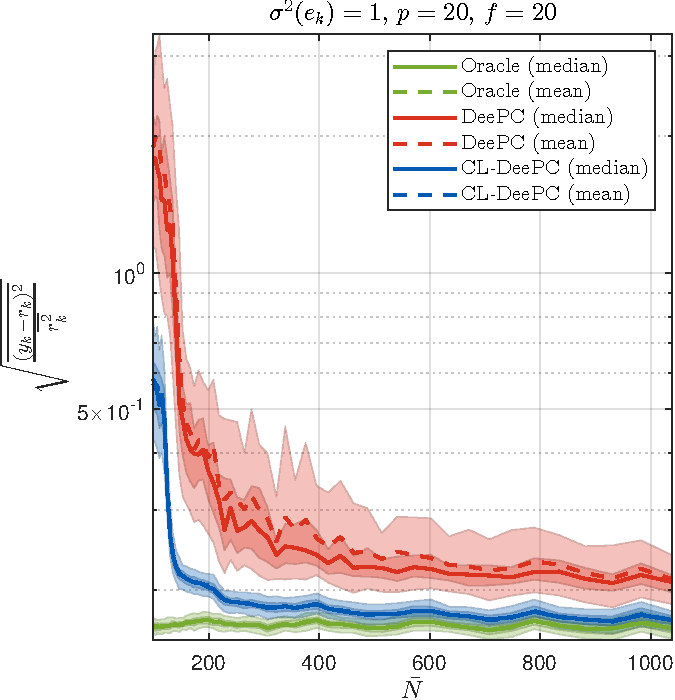
\includegraphics[width=\columnwidth]{results/figures/Varying_Nbar_99-1039-50_p_20_f_20_Re_1_Ru_1_Rdu_0_Q_100_R_0_dR_10.pdf}    % The printed column  
\caption{Increasingly narrow regions around the median contain 80\% and 40\% of the data.}  % width is 8.4 cm.
\label{fig:varying_Nbar}                                 % Size the figures 
\end{center}                                 % accordingly.
\end{figure}
% -----------------------------------------------------------

\subsection{Noise level: $\sigma^2(e_k)$}
% ------------------------- Figure --------------------------
\begin{figure}[b!]
\begin{center}
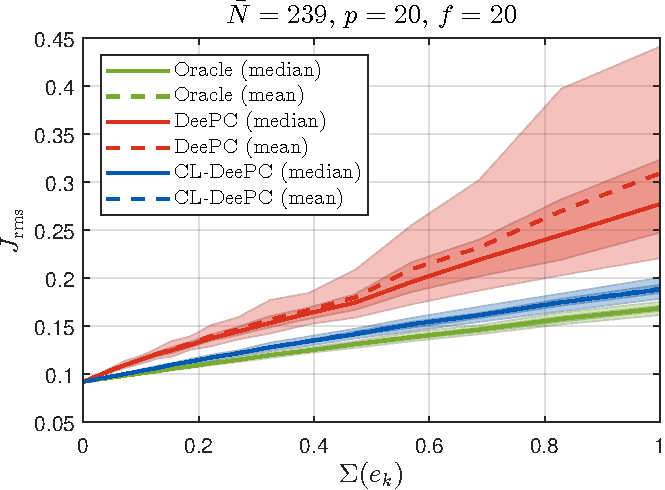
\includegraphics[width=\columnwidth]{results/figures/Varying_Re_0.0001-1-50_Nbar_239_p_20_f_20_Ru_1_Rdu_0_Q_100_R_0_dR_10.pdf}    % The printed column 
\caption{Increasingly narrow regions around the median contain 80\% and 40\% of the data.}  % width is 8.4 cm.
\label{fig:varying_Re}                                 % Size the figures 
\end{center}                                 % accordingly.
\end{figure}
% -----------------------------------------------------------

\subsection{Past data window lengths: $p=f$}
% ------------------------- Figure --------------------------
\begin{figure}[b!]
\begin{center}
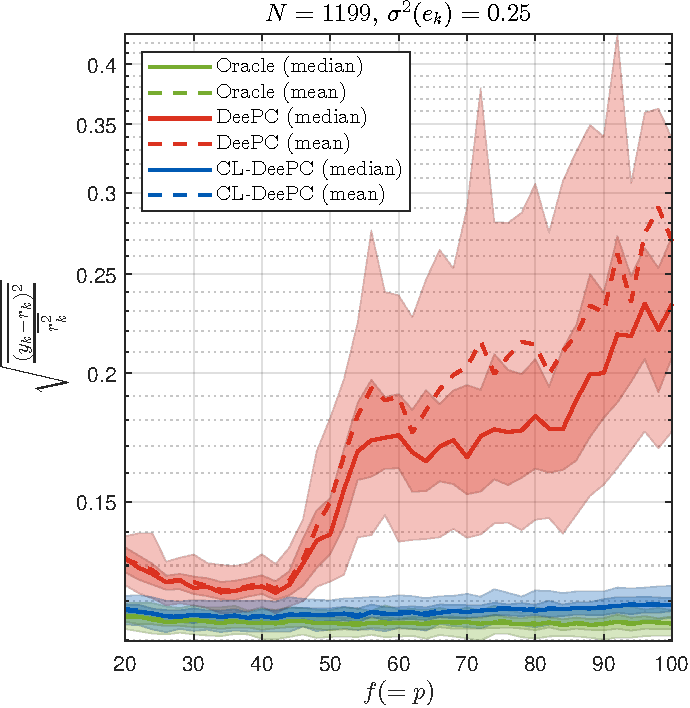
\includegraphics[width=\columnwidth]{results/figures/Varying_pf_20-100-41_Nbar_1199_Re_0.25_Ru_1_Rdu_0_Q_100_R_0_dR_10.pdf}    % The printed column 
\caption{Increasingly narrow regions around the median contain 80\% and 40\% of the data.}  % width is 8.4 cm.
\label{fig:varying_Re}                                 % Size the figures 
\end{center}                                 % accordingly.
\end{figure}
% -----------------------------------------------------------